\documentclass[10pt] {beamer}
\usepackage[utf8x]{inputenc}
\usepackage[english]{babel}
\usetheme{Berlin}
\usepackage{thumbpdf}
\usepackage{wasysym}
\usepackage{ucs}
\beamertemplatenavigationsymbolsempty
%\usepackage {pgf,pgfarrows,pgfnodes,pgfautomata,pgfheaps,pgfshade}
\usepackage {verbatim}
\pdfinfo
{
    /Title       (Build facili con CMake)
    /Creator     (TeX)
    /Author      (Carlo Nicolini)
}


\title{Build facili con CMake}
\subtitle{Il sistema di build -definitivo-}
\author{Carlo Nicolini}
\date{\today}

\begin {document}
\frame{\titlepage}

%%%%%%%%%%%%%%%%%%%%%%%%%%%%%%%%%%%%%%%%%
%%%%%%%%%% INTRODUZIONE %%%%%%%%%%%%%%%%%
%%%%%%%%%%%%%%%%%%%%%%%%%%%%%%%%%%%%%%%%%

\section{Introduzione}
\begin{frame}
\frametitle{Motivazioni}
Un sistema di build per C/C++ ci permette di essere più efficienti, produttivi e chiari.
Vogliamo un sistema di build che ci permetta
\begin{itemize}
\item<1-> Portabilità su molti O.S.
\item<2-> Gestione di molti tipi di build diversa
\item<3-> Supporto a librerie esterne
\item<4-> Facilità di mantenimento di un progetto
\item<5-> Chiarezza ed intuitività, \textbf{velocità} di build
\item<6-> Build parallele
\item<7-> Miglior rapporto con chi userà il nostro codice
\item<8-> Packing, unit testing, profiling e debugging ALL-IN-ONE
\end{itemize}
\end{frame}

%%%%%%%%%%%%%%%%%%%%%%%%%%%%%%%%%%%%%%%%%%%%%%%%%%%%%%%%%%%%%%%%%%%%%%%%%%%%%%%%
\begin{frame}
\frametitle{Sistemi di build}
Un sistema di build si occupa di generare eseguibili/librerie partendo dai sorgenti \footnote{\url{http://www.cs.virginia.edu/~dww4s/articles/build_systems.html}}
\begin{figure}[htb]
 \centering
 
\includegraphics[width=0.6\textwidth]{images/hello_digraph.png}
\end{figure}
Problema delle dipendenze = punti d'articolazione su grafo DAG.

Limite al parallelismo (CMake supporta build multiprocessore).
\end{frame}

%%%%%%%%%%%%%%%%%%%%%%%%%%%%%%%%%%%%%%%%%%%%%%%%%%%%%%%%%%%%%%%%%%%%%%%%%%%%%%%%
\begin{frame}[fragile]
\frametitle{In passato}
In passato sono apparsi tanti sistemi, ognuno con i suoi pro e contro. Dimentichiamo la compilazione manuale (anni 70)
\begin{verbatim}
 gcc -c mylibrary.cpp mylibrary.h -o mylibrary.o
\end{verbatim}
e passiamo ai sistemi di build automatici:

\begin{itemize}
\item<1-> Scons \textit{basato su Python, cross-platform}
\item<2-> Autotools \textit{ molto usato, sintassi complicata (Autohell), solo Unix }
\item<3-> Jam \textit{ (cross-platform,cross-language), buggy, poco automatico}\footnote{\url{http://en.wikipedia.org/wiki/Perforce_Jam}}
\item<4-> Waf \textit{ python un singolo file da redistribuire \footnote{\url{http://docs.waf.googlecode.com/git/book_17/waf.pdf}}}
\item<5-> Altri?
\end{itemize}
\end{frame}

%%%%%%%%%%%%%%%%%%%%%%%%%%%%%%%%%%%%%%%%%%%%%%%%%%%%%%%%%%%%%%%%%%%%%%%%%%%%%%%%

\begin{frame}
\frametitle{CMake}
Un sistema di build moderno gestisce building, testing e packaging tutto insieme, scritto in C++, supporta progetti C/C++\footnote{\url{www.cmake.org}}.
\begin{itemize}
		\item<1-> Sistema di meta-make, multiprogetto (targets)
		\item<2-> Supporto a tanti ambienti di sviluppo (IDE) tramite \emph{generatori}\footnote{\url{http://www.cmake.org/cmake/help/v2.8.8/cmake.html\#section\_Generators}}: 

Kdevelop3, Eclipse, XCode, Code::Blocks ,VisualStudio, Makefiles (Unix, NMake, Borland, MinGW, Cygwin)

		\item<3-> Cross plattform (veramente).
		\item<4-> Dipendenze soddisfatte sempre (veramente).
		\item<5-> Un linguaggio di scripting che da libertà (vera).
		\begin{itemize}
			\item<6-> \texttt{\#define } a compile-time tramite variabili scriptabili.
			\item<7-> Supporto menu Gnome, icone e creazione setup personalizzati.
			\item<8-> Centinaia di librerie esterne supportate.
		\end{itemize}
		\item<9-> \textbf{Out-of-source} builds: fare una build senza ``sporcare'' la codebase
\end{itemize}
\end{frame}

%%%%%%%%%%%%%%%%%%%%%%%%%%%%%%%%%%%%%%%%%%%%%%%%%%%%%%%%%%%%%%%%%%%%%%%%%%%%%%%%

\begin{frame}[fragile]
 \frametitle{Moduli supportati}
\begin{block}{Forniti insieme a CMake}
 ALSA, Armadillo, ASPELL, AVIFile, BISON, \textbf{BLAS}, \textbf{Boost}, Bullet, BZip2, CABLE, 
 Coin3D, \textbf{CUDA}, Cups, CURL, Curses, CVS, CxxTest, \textbf{Cygwin}, Dart, DCMTK, 
 DevIL, Doxygen, EXPAT, FLEX, FLTK2, FLTK, Gettext,
 GIF, Git, GLU, \textbf{GLUT}, Gnuplot, GnuTLS, GTest, GTK2, GTK, HDF5, HSPELL, 
 HTMLHelp, \textbf{ImageMagick}, ITK, Jasper, Java, JNI, JPEG, KDE3, \textbf{KDE4}, LAPACK, LATEX, 
 LibArchive, LibXml2, LibXslt, Lua50, Lua51, Matlab, MFC, Motif, MPEG2, MPEG, MPI, 
 OpenAL, OpenGL, OpenMP, OpenSceneGraph, OpenSSL, OpenThreads, osgAnimation,  
PackageMessage, \textbf{Perl}, PerlLibs, PHP4, PhysFS, Pike, PkgConfig, PNG, PostgreSQL,  PythonInterp, 
 \textbf{PythonLibs}, Qt3, \textbf{Qt4}, QuickTime, Ruby, SDL, SelfPackers, Subversion, 
 SWIG, TCL, Tclsh, TclStub, \textbf{Threads}, TIFF, UnixCommands, VTK, Wget, 
 Wish, wxWidgets, wxWindows, X11, XMLRPC, ZLIB
\end{block}
e tanti altri si trovano sul web
\end{frame}

%%%%%%%%%%%%%%%%%%%%%%%%%%%%%%%%%%%%%%%%%%%%%%%%%%%%%%%%%%%%%%%%%%%%%%%%%%%%%%%%%
\begin{frame}[fragile]
\frametitle{CMake tree e primi passi}

\begin{block}{Tree di un progetto base}
\begin{itemize}
\item \textbf{src}/
\begin{itemize}
	\item myapp.cpp
	\item myapp.h
	\item CMakeLists.txt
\end{itemize}
\item \textbf{build}/
\item \emph{cmake}/
\item \emph{doc}/
\item \emph{deps}/
\item \emph{doc}/
\item CMakeLists.txt
\end{itemize}
\end{block}
\end{frame}

%%%%%%%%%%%%%%%%%%%%%%%%%%%%%%%%%%%%%%%%%%%%%%%%%%%%%%%%%%%%%%%%%%%%%%%%%%%%%%%%%%%%%%%%%%%%%%%%

\begin{frame}[fragile]
\frametitle{Opzioni di compilazione}
\begin{itemize}
 \item Definizione di opzioni di compilazione
 \item Switch su opzioni
 \item Switch su compilatori
 \item Switch su librerie
 \item etc...
\end{itemize}

\begin{verbatim}
//CMakeLists.txt
option(MyOption "MyOption" OFF)
//Da linea di comando
cmake -DMyOption=ON .
\end{verbatim}

Esempio 07-qt+opengl
\end{frame}


%%%%%%%%%%%%%%%%%%%%%%%%%%%%%%%%%%%%%%%%%%%%%%%%%%%%%%%%%%%%%%%%%%%%%%%%%%%%%%%%

\begin{frame}[fragile]
\frametitle{Compatibilità con versioni precedenti}
\begin{itemize}
\item Molto importante impostare la compatibilita con le versioni precedenti, cambi di sintassi, bug-fix e nuovi moduli.
\item Mantenere sempre CMake all'ultima versione (attuale 2.8.10).
\item Variabile di sistema apposita.
\end{itemize}
\begin{verbatim}
 CMAKE_MINIMUM_REQUIRED(VERSION 2.6.0 FATAL_ERROR)
\end{verbatim}
\end{frame}

%%%%%%%%%%%%%%%%%%%%%%%%%%%%%%%%%%%%%%%%%%%%%%%%%%%%%%%%%%%%%%%%%%%%%%%%%%%%%%%%%%%%%%%%%%%%%%%%

\begin{frame}[fragile]
	\frametitle{Variabili in CMake}
	\begin{itemize}
		\item Non serve dichiararle (stringa vuota se non esistono).
		\item Atipizzate.
		\item SET crea e modifica variabili.
		\item SEPARATE\_ARGUMENTS spezza argomenti separati da spazio in una LIST.
		\item Da Cmake $>$ 2.6 variabili scoped.
		\item Dereferenza stile bash (attenzione all'assegnazione!) 
		\begin{alertblock}{Attenzione}
			\begin{small}
			\begin{verbatim}
			FOO="fooval"
			BAR=FOO
			QUX=${FOO}
		\end{verbatim}
		\end{small}
		BAR e QUX hanno valori diversi! (tutte variabili sono stringhe)
		\end{alertblock}
\end{itemize}
\end{frame}

%%%%%%%%%%%%%%%%%%%%%%%%%%%%%%%%%%%%%%%%%%%%%%%%%%%%%%%%%%%%%%%%%%%%%%%%%%%%%%%%%%%%%%%%%%%%%%%%

\begin{frame}[fragile]
 \frametitle{Comando SET}
Settare una variabile in CMake con il comando \textbf{SET}\footnote{I comandi sono case-insensitive}
\begin{block}{Esempio di uso del comando SET}
\begin{small}
\begin{verbatim}
SET(USE_BOOST_LIBRARIES "ON")
message(STATUS "Are you using Boost libraries? 
    ${USE_BOOST_LIBRARIES})

SET( MyProjectHeaders "Ciccio.h Pippo.h Mimmo.h")
set( MyProjectSources "Ciccio.cpp Mimmo.cpp" )
\end{verbatim}
\end{small}
\end{block}
\end{frame}


%%%%%%%%%%%%%%%%%%%%%%%%%%%%%%%%%%%%%%%%%%%%%%%%%%%%%%%%%%%%%%%%%%%%%%%%%%%%%%%%%%%%%%%%%%%%%%%%

\begin{frame}[fragile]
	\frametitle{Sintassi}
\begin{itemize}
 \item Costrutto condizionale IF
	\begin{verbatim}
	IF ( expression )
	...
	ELSE ( expression )
	...
	ENDIF ( expression )
	\end{verbatim}
\item Costrutto FOREACH ( comodo per liste)
	\begin{verbatim}
	FOREACH ( loopvariable )
	...
	ENDFOREACH ( loopvariable )
	\end{verbatim}
\item Ciclo WHILE
	\begin{verbatim}
	WHILE ( condition )
	...
	ENDWHILE ( condition )
	\end{verbatim}
\end{itemize}
\end{frame}

%%%%%%%%%%%%%%%%%%%%%%%%%%%%%%%%%%%%%%%%%%%%%%%%%%%%%%%%%%%%%%%%%%%%%%%%%%%%%%%%%%%%%%%%%%%%%%%%

\begin{frame}[fragile]
\frametitle{Esempio di foreach e wildcards su files}
Il comando \texttt{file} è una chiamata al sistema
\begin{block}{Esempio}
\begin{small}
\begin{verbatim}
file(GLOB mytestfiles "test*.cpp")
foreach(testfile ${mytestfiles})
  message(STATUS "This is a test file ${testfile}")
endforeach(testfile ${mytestfiles })
\end{verbatim}
\end{small}
\end{block}
\end{frame}

%%%%%%%%%%%%%%%%%%%%%%%%%%%%%%%%%%%%%%%%%%%%%%%%%%%%%%%%%%%%%%%%%%%%%%%%%%%%%%%%%%%%%%%%%%%%%%%%

\begin{frame}[fragile]
\frametitle{\emph{Switch} condizionali di sistema}
\begin{verbatim}
IF ( MSVC )
ENDIF ( MSVC )

IF (WIN32)
ENDIF (WIN32)
 		
IF ( UNIX )
ENDIF (UNIX)
 		
IF (APPLE)
ENDIF (APPLE)
\end{verbatim}
\begin{itemize}
\item Tutte le variabili sono scoped nel singolo CMakeLists.txt
\item Non esiste un costrutto \textbf{switch}
\end{itemize}
\end{frame}

%%%%%%%%%%%%%%%%%%%%%%%%%%%%%%%%%%%%%%%%%%%%%%%%%%%%%%%%%%%%%%%%%%%%%%%%%%%%%%%%%%%%%

\begin{frame}[fragile]
\frametitle{ Espressioni regolari}

\begin{block}{Regexp}
\begin{verbatim}
STRING( REGEX MATCH ... )
STRING (REGEX MATCHALL ... )
STRING(REGEX REPLACE ... )
\end{verbatim}
\end{block}

Esempio:
\begin{block}{Esempio regex}
\begin{small}
\begin{verbatim}
SET(test "hello world ! catch: me if you can")
STRING(REGEX REPLACE ".*catch: ([^ ]+).*" "\\1" 
  result "${test}" )
MESSAGE(STATUS "result= ${result}")
\end{verbatim}
\end{small}
\end{block}
stampa a stdout:
\begin{verbatim}
  -- result= me
\end{verbatim}
(il \texttt{--} è stampato ad ogni riga di default)
\end{frame}


%%%%%%%%%%%%%%%%%%%%%%%%%%%%%%%%%%%%%%%%%%%%%%%%%%%%%%%%%%%%%%%%%%%%%%%%%%%%%%%%

\begin{frame}
\frametitle{Cmake cache}
\begin{itemize}
\item CMake salva le variabili non variate in un file CMakeCache.txt
\item Veloce su Unix, lento su Windows (MSVC)
\item Utile ripulire la cache
\end{itemize}

\begin{itemize}
\item \texttt{rm CMakeCache.txt}, oppure
\item Cancellare manualmente il file \texttt{CMakeCache.txt}
\item Rigenerare il progetto
\end{itemize}

\end{frame}

%%%%%%%%%%%%%%%%%%%%%%%%%%%%%%%%%%%%%%%%%%%%%%%%%%%%%%%%%%%%%%%%%%%%%%%%%%%%%%%%

\begin{frame}[fragile]
\frametitle{Gestione di Debug e Release}
\begin{itemize}
\item<1-> Una variabile definisce il tipo di build
\item<2->
\begin{verbatim}
SET(CMAKE_BUILD_TYPE XXX)
\end{verbatim}
    \begin{itemize}
    \item \texttt{Debug}
    \item \texttt{Release}
    \item \texttt{RelWithDebInfo}
    \item \texttt{MinSizeRel}
    \item \texttt{Profile}
    \end{itemize}
\item<3-> oppure da linea di comando:
\begin{verbatim}
cmake -DCMAKE_BUILD_TYPE=Debug .
\end{verbatim}

\item<4-> \texttt{Debug} $\rightarrow$ gdb+valgrind, grosse dimensioni
\item<5-> \texttt{Profile} utile quando accoppiata con gprof/KCacheGrind
\item<6-> Deploy si effettua sempre in \texttt{Release}
\end{itemize}
\end{frame}

%%%%%%%%%%%%%%%%%%%%%%%%%%%%%%%%%%%%%%%%%%%%%%%%%%%%%%%%%%%%%%%%%%%%%%%%%%%%%%%%

\begin{frame}[fragile]
 \frametitle{Informazioni revisione compile-time}
Viene in aiuto il modulo FindSubversion (ripulire cache prima)

\begin{block}{Working copy informations}
\begin{small}
\begin{verbatim}
FIND_PACKAGE(Subversion)
IF(SUBVERSION_FOUND)
Subversion_WC_INFO(${PROJECT_SOURCE_DIR} Project)
MESSAGE("Current revision is ${Project_WC_REVISION}")
Subversion_WC_LOG(${PROJECT_SOURCE_DIR} Project)
MESSAGE("Last changed log is ${Project_LAST_CHANGED_LOG}")
ENDIF(SUBVERSION_FOUND)
\end{verbatim}
\end{small}
\end{block}

Usare ADD\_DEFINITIONS:

%\begin{block}
%\begin{small}
%\begin{verbatim}
%ADD_DEFINITIONS(-DREV_NUMBER=
%"${SUBVERSION_REPO_REVISION}")
%\end{verbatim}
%\end{small}
%\end{block}

\end{frame}

%%%%%%%%%%%%%%%%%%%%%%%%%%%%%%%%%%%%%%%%%%%%%%%%%%%%%%%%%%%%%%%%%%%%%%%%%%%%%%%%

\begin{frame}[fragile]
 \frametitle{Generare la documentazione}
Aggiungere un target \texttt{doc} ed usare \texttt{FindDoxygen.cmake}
\begin{block}{Esempio}
\begin{small}
\begin{verbatim}
find_package(Doxygen)
if(DOXYGEN_FOUND)
configure_file(${CMAKE_CURRENT_SOURCE_DIR}/Doxyfile 
    ${CMAKE_CURRENT_BINARY_DIR}/Doxyfile @ONLY)
# Aggiunge un target doc al Makefile 
add_custom_target(doc
${DOXYGEN_EXECUTABLE} ${CMAKE_CURRENT_BINARY_DIR}/Doxyfile
WORKING_DIRECTORY ${CMAKE_CURRENT_BINARY_DIR}
COMMENT "Generating API documentation with Doxygen" 
    VERBATIM )
endif(DOXYGEN_FOUND)
\end{verbatim}
\end{small}
\end{block}
Vedi \url{http://bit.ly/9eel8b}
\end{frame}

%%%%%%%%%%%%%%%%%%%%%%%%%%%%%%%%%%%%%%%%%%%%%%%%%%%%%%%%%%%%%%%%%%%%%%%%%%%%%%%%
%%%%%%%%%%%%%%%%%%%%%%%%%%%%%%%%%%%%%%%%%%%%%%%%%%%%%%%%%%%%%%%%%%%%%%%%%%%%%%%%
\section{Esempi e tutorial}
%%%%%%%%%%%%%%%%%%%%%%%%%%%%%%%%%%%%%%%%%%%%%%%%%%%%%%%%%%%%%%%%%%%%%%%%%%%%%%%%
%%%%%%%%%%%%%%%%%%%%%%%%%%%%%%%%%%%%%%%%%%%%%%%%%%%%%%%%%%%%%%%%%%%%%%%%%%%%%%%%

\begin{frame}[fragile]
\frametitle{HelloWorld eseguibile}

\begin{block}{Hello world!}
\begin{small}
\begin{verbatim}
#Creiamo il nome del progetto
PROJECT( helloworld )
# Impostiamo la variabile hello_SRCS a contenere la hello.cpp
SET( hello\_SRCS hello.cpp )
# Crea l'eseguibile di nome hello dal file contenuto 
# nella variabile hello\_SRCS
ADD\_EXECUTABLE( hello \$\{hello\_SRCS\} )
\end{verbatim}
\end{small}
\end{block}

\emph{Esempio 01-helloworld}
\end{frame}

%%%%%%%%%%%%%%%%%%%%%%%%%%%%%%%%%%%%%%%%%%%%%%%%%%%%%%%%%%%%%%%%%%%%%%%%%%%%%%%%

\begin{frame}[fragile]
	\frametitle{Creazione librerie statica/dinamica}
\begin{verbatim}
#Creiamo il nome del progetto
PROJECT( mylibrary )
# Impostiamo la variabile mylibrary_SRCS a contenere tutti i 
# file che definiscono la libreria
SET( mylibrary_SRCS Foo.cpp Bar.cpp Qux.cpp)
# Crea una libreria STATICA (di default in CMake) 
# in Linux con gcc genera un file libMyLibrary.a
ADD_LIBRARY( MyLibrary ${mylibrary_SRCS} )
# in Linux con gcc genera un file libMyLibrary.so
ADD_LIBRARY( myLibrary ${mylibrary_SRCS} )
\end{verbatim}

\emph{Esempi 02-staticlib, 03-dynamiclib}

\end{frame}


\begin{frame}[fragile]
 \frametitle{Generazione grafo delle dipendenze}
CMake supporta la generazione visual del grafo delle dipendenze fra files, sfruttando il pacchetto di graph-drawing \textbf{Graphviz}
\begin{verbatim}
cmake --graphviz=dependencies.dot .
dot -Tpng dependencies.dot > dependencies.png
\end{verbatim}
\begin{figure}[htb]
 \centering
 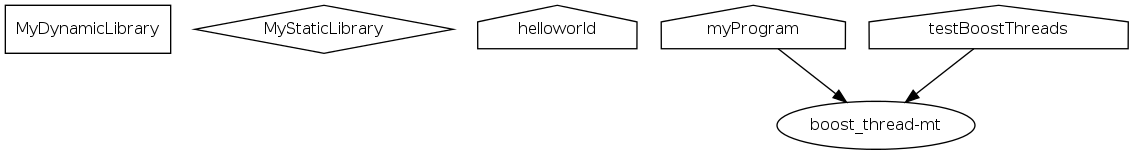
\includegraphics[width=0.9\textwidth]{images/dependencies.png}
\end{figure}
\end{frame}


%%%%%%%%%%%%%%%%%%%%%%%%%%%%%%%%%%%%%%%%%%%%%%%%%%%%%%%%%%%%%%%%%%%%%%%%%%%%%%%%
%%%%%%%%%%%%%%%%%%%%%%%%%%%%%%%%%%%%%%%%%%%%%%%%%%%%%%%%%%%%%%%%%%%%%%%%%%%%%%%%

\begin{frame}[fragile]
\frametitle{Boost}
Boost è una libreria estensione del C++:
\begin{itemize}
\item ''...one of the most highly regarded and expertly designed C++ library projects in the world.''
— Herb Sutter and Andrei Alexandrescu, C++ Coding Standards
\item ''Item 55: Familiarize yourself with Boost.''
— Scott Meyers, Effective C++, 3rd Ed.
\end{itemize}
Boost contiene supporto headers-only e anche librerie bimap, containers generici, interfacce IO, socket, \textbf{threading} e molto altro ancora.
\end{frame}

\begin{frame}[fragile]
 \frametitle{CMake + Boost}
Nel CMakeLists.txt di base
\begin{verbatim}
# Set the needed boost libraries 
set(BOOST_LIBS thread date_time system program_options 
  filesystem regex serialization iostreams)
set(Boost_USE_STATIC_LIBS        ON)
set(Boost_USE_MULTITHREADED      ON)
set(Boost_USE_STATIC_RUNTIME    OFF)

find_package(Boost COMPONENTS ${BOOST_LIBS} REQUIRED)
include_directories(${Boost_INCLUDE_DIR})
find_package(Threads REQUIRED)
\end{verbatim}

\end{frame}

%%%%%%%%%%%%%%%%%%%%%%%%%%%%%%%%%%%%%%%%%%%%%%%%%%%%%%%%%%%%%%%%%%%%%%%%%%%%

\begin{frame}[fragile]
 \frametitle{CMake + Boost}
Linkare una libreria a Boost
\begin{verbatim}
add_library(FooBar Foo.cpp Bar.cpp)
target_link_libraries(FooBar 
  ${BOOST_LIBRARIES})
\end{verbatim}
Linkare un eseguibile a Boost:
\begin{verbatim}
add_executable(myApplication myApplication.cpp 
    Foo.cpp Bar.cpp)
target_link_libraries(myApplication(myApplication 
    ${BOOST_LIBRARIES})
\end{verbatim}
Viene \textbf{automagicamente} selezionata la versione della libreria corretta:
\begin{itemize}
\item \textbf{build statica multithread} \verb_/usr/lib/libboost_\verb_thread-mt.a_
\item \textbf{build dinamica non-multithread} \verb_/usr/lib/libboost_\verb_thread.so_
\end{itemize}
\end{frame}
%%%%%%%%%%%%%%%%%%%%%%%%%%%%%%%%%%%%%%%%%%%%%%%%%%%%%%%%%%%%%%%%%%%%%%%%%%%%%%%%

\section{Supporto a librerie esterne}
\begin{frame}[fragile]
 \frametitle{Supporto a OpenMP}
\begin{footnotesize}
\begin{verbatim}
include(FindOpenMP)
if(OPENMP_FOUND)
   set(CMAKE_CXX_FLAGS "${CMAKE_CXX_FLAGS} 
         ${OpenMP_CXX_FLAGS}")
   set(CMAKE_EXE_LINKER_FLAGS "${CMAKE_EXE_LINKER_FLAGS} 
         ${OpenMP_EXE_LINKER_FLAGS}")
endif()
\end{verbatim}
\end{footnotesize}
\begin{itemize}
 \item Sceglie il flag appropriato del compilatore (\texttt{-fopenmp} su g++ , \texttt{-openmp} su Intel icc, \texttt{/openmp} su MSVC )
 \item Problemi con \texttt{vcompd.dll}, modificare il file manifest con MSVC9 (2008)\footnote{\url{http://kitware.com/blog/home/post/4}}
\item \url{http://public.kitware.com/Bug/view.php?id=12964}
\end{itemize}

\end{frame}


\begin{frame}[fragile]
\frametitle{CMake e Qt}
CMake interagisce molto bene con Qt (e viceversa)
\begin{footnotesize}
\begin{verbatim}
set(QT_MIN_VERSION "4.6.0")
set(QT_USE_QTMAIN TRUE)
set(QT_USE_OPENGL TRUE)
find_package(Qt4 4.6.0 COMPONENTS QtGui QtCore 
	    QtOpenGL REQUIRED )
INCLUDE(${QT_USE_FILE})
\end{verbatim}
\end{footnotesize}
\end{frame}

%%%%%%%%%%%%%%%%%%%%%%%%%%%%%%%%%%%%%%%%%%%%%%%%%%%%%%%%%%%%%%%%%%%%%%%%%%%%%%%%

\begin{frame}[fragile]
 \frametitle{CMake e Qt}
\begin{block}{Ingredienti}

\begin{itemize} 
\item <1-> Cercare Qt4 nel sistema
\begin{verbatim}
Find_Package(Qt4 REQUIRED)
INCLUDE( ${QT_USE_FILE} )
\end{verbatim}
\item <2-> Indicare i sorgenti .cpp ed i forms .ui
\begin{verbatim}
QT4_WRAP_CPP, QT4_WRAP_UI 
\end{verbatim}
\item <3-> Indicare il file risorsa (icone, suoni, immagini etc)
\begin{verbatim}
QT4_ADD_RESOURCES
\end{verbatim}
\item<4-> Linkare il tutto ed includere le directory di Qt
\begin{small}
\begin{verbatim}
link_libraries(${QT_QTCORE_LIBRARY} ${QT_QTGUI_LIBRARY} )
include_directories(${QT_INCLUDE_PATH} 
  ${QT_QTGUI_INCLUDE_DIR}
  ${QT_QTCORE_INCLUDE_DIR} )
\end{verbatim}
\end{small}
\end{itemize}

\end{block}
\end{frame}

\begin{frame}[fragile]
 \frametitle{Semplice progettino con Qt}
\begin{block}{Esempio di Qt}
 \begin{small}
\begin{verbatim}
PROJECT( pfrac )
FIND_PACKAGE( Qt4 REQUIRED )
INCLUDE( ${QT_USE_FILE} )
SET( pfrac_SRCS main.cpp client.h client.cpp )
SET( pfrac_MOC_HEADERS client.h )
QT4_ADD_RESOURCES( pfrac_SRCS 
     ${PROJECT_SOURCE_DIR}/pfrac.qrc )
QT4_WRAP_CPP( pfrac_MOC_SRCS 
     ${pfrac_MOC_HEADERS} )
ADD_EXECUTABLE( pfrac ${pfrac_SRCS} $
{pfrac_MOC_SRCS} 
TARGET_LINK_LIBRARIES( pfrac ${QT_LIBRARIES} )
\end{verbatim}
\end{small}
\end{block}

\end{frame}


%%%%%%%%%%%%%%%%%%%%%%%%%%%%%%%%%%%%%%%%%%%%%%%%%%%%%%%%%%%%%%%%%%%%%%%%%%%%%%%%%%%%%%%%%%%%%%%%

\begin{frame}[fragile]
 \frametitle{CMake + OpenGL}
Esistono diversi modi di supportare OpenGL con CMake, sono tutti cross-platform
\begin{itemize}
 \item FindOpenGL.cmake
 \item FindGlut.cmake
\end{itemize}

Su Linux è molto facile (previa installazione di GLU/GLUT/FreeGLUT)
\begin{block}{Librerie OpenGL}
 \begin{small}
  \begin{verbatim}
find_package(OpenGL REQUIRED)
include_directories(${OPENGL_INCLUDE_DIR})
find_package(GLUT REQUIRED)
set(GL_LIBS ${OPENGL_LIBRARIES} ${GLUT_LIBRARIES})
...
target_link_libraries(myApp ${GL_LIBS})
\end{verbatim}
 \end{small}
\end{block}


\end{frame}

%%%%%%%%%%%%%%%%%%%%%%%%%%%%%%%%%%%%%%%%%%%%%%%%%%%%%%%%%%%%%%%%%%%%%%%%%%%%%%%%%%%%%%%%%%%%%%%%

\section{Creazione pacchi con CPack}
\begin{frame}
\frametitle{CPack}
CPack è il progetto cugino di CMake con cui è strettamente integrato e permette di creare pacchi:
\begin{itemize}
\item Linux generici ( .sh, .tgz )
\item Distro-based ( .deb, .rpm, )
\item OSX (creazione .app o dischi .dmg )
\item Windows (creazione setup.exe grazie a NSIS installer e 7Zip )
\end{itemize}
\begin{itemize}
\item Pacchi architettura-specifici
\item Cross compilazione!
\end{itemize}
\end{frame}

%%%%%%%%%%%%%%%%%%%%%%%%%%%%%%%%%%%%%%%%%%%%%%%%%%%%%%%%%%%%%%%%%%%%%%%%%%%%%%%%%%%%%%%%%%%%%%%%
\begin{frame}[fragile]
\frametitle{CPack}
Creazione di un installer per una libreria  \textbf{MyLib} \footnote{\url{http://cmake.org/Wiki/CMake:Component_Install_With_CPack}}
\begin{verbatim}
install(TARGETS MyLib 
  ARCHIVE
  DESTINATION lib)

install(TARGETS MyLibApp
  RUNTIME
  DESTINATION bin)

install(FILES MyLibrary.h
  DESTINATION include)
\end{verbatim}
\end{frame}

%%%%%%%%%%%%%%%%%%%%%%%%%%%%%%%%%%%%%%%%%%%%%%%%%%%%%%%%%%%%%%%%%%%%%%%%%%%%%%%%%%%%%%%%%%%%%%%%
\begin{frame}[fragile]
 \frametitle{Installer per la libreria MyLib}
\begin{verbatim}
set(CPACK_PACKAGE_NAME "MyLib")
set(CPACK_PACKAGE_VENDOR "CMake.org")
set(CPACK_PACKAGE_DESCRIPTION_SUMMARY "Esempio CPack")
set(CPACK_PACKAGE_VERSION "1.0.0")
set(CPACK_PACKAGE_VERSION_MAJOR "1")
set(CPACK_PACKAGE_VERSION_MINOR "0")
set(CPACK_PACKAGE_VERSION_PATCH "0")
set(CPACK_PACKAGE_INSTALL_DIRECTORY "CPack Example")

# Ultimo comando da includere nel CMakeLists.txt
include(CPack)
\end{verbatim}
\end{frame}

%%%%%%%%%%%%%%%%%%%%%%%%%%%%%%%%%%%%%%%%%%%%%%%%%%%%%%%%%%%%%%%%%%%%%%%%%%%%%%%%%%%%%%%%%%%%%%%%%%%%

\begin{frame}
\frametitle{Hands on CMake/CPack}

Ho preparato alcune risorse per potere meglio capire i concetti 
\begin{block}{Pacchetti necessari}
\texttt{sudo apt-get git install build-essentials cmake libbboost-dev}
\end{block}

\begin{block}{GitHub repository}
\texttt{git clone https://github.com/CarloNicolini/cmake-slides.git} 
\end{block}

\end{frame}

%%%%%%%%%%%%%%%%%%%%%%%%%%%%%%%%%%%%%%%%%%%%%%%%%%%%%%%%%%%%%%%%%%%%%%%%%%%%%%%%%%%%%%%%%%%%%%%%%%%%

\begin{frame}
\frametitle{Risorse online}
\begin{thebibliography}{10}

\beamertemplatearticlebibitems

\bibitem{CMake mailing list}
Mailing list ufficiale degli utenti di CMake
\newblock{\url{http://www.cmake.org/mailman/listinfo/cmake}}

\bibitem{stackoverflow}
Sito di domande e risposte, frequentato da molti utenti di CMake
\newblock{\url{www.stackoverflow.com}}

\bibitem{Cmake tutorial}
CMake tutorial online
\newblock{\url{http://www.cmake.org/cmake/help/cmake_tutorial.html}}

\bibitem{Mastering CMake}
Il libro ufficiale, insostituibile
\newblock{\url{http://www.kitware.com/products/books/CMakeBook.html}}
\end{thebibliography}
\end{frame}

\frame{
    \vspace{2cm}
    {\huge Domande ?}

    \vspace{3cm}
    \begin{flushright}
    Carlo Nicolini

    \structure{\footnotesize{nicolini.carlo@gmail.com}}
    \end{flushright}
}

\end{document}
